\documentclass[article,A4,12pt]{llncs}
\usepackage[T1]{fontenc}
\usepackage{amsmath}
\usepackage{amssymb}
\usepackage{amsfonts}
\usepackage{mathrsfs, bm}

\usepackage{graphicx}
\usepackage{tabularx}
\usepackage{subfig}
\usepackage{epsf,times}
\usepackage{color}
\usepackage{wrapfig}
\usepackage{cases}
\usepackage{multicol}

\usepackage[T1]{fontenc}
%\newcommand{\tmname}[1]{\textsc{#1}}
%\newcommand{\tmop}[1]{\ensuremath{\operatorname{#1}}}
%\newcommand{\tmsamp}[1]{\textsf{#1}}
%\newcommand{\tmtextsc}[1]{{\scshape{#1}}}
%\newcommand{\tmtextsl}[1]{{\slshape{#1}}}
%\newcommand{\tmtexttt}[1]{{\ttfamily{#1}}}

\leftmargin=0.0cm
\oddsidemargin=0.5cm
\evensidemargin=0.5cm
\topmargin=0cm
\textwidth=16.0cm
%\textheight=21.5cm
\textheight=20.0cm
\pagestyle{plain}
\setlength{\columnsep}{20pt}

\def\m{\mathbf{m}}
\def\H{\mathbf{H}}
\def\E{\mathbf{E}}
\newcommand{\vepsi}{{\varepsilon}}
\def\hnorm#1#2{\vert\,#1\,\vert_{#2}}
\newcommand{\R}{{\mathbb R}}
\newcommand{\Sph}{{\mathbb S}}
\def\x{\mathbf{x}}
\def\hvec{\overline{\mathbf{h}}}
\def\evec{\overline{\mathbf{e}}}

\newcommand{ \etal}{\mbox{\emph{et al. }}}

\newcommand\vect[1]{\mbf{#1}}
\newcommand{\mbf}[1]{\mbox{\boldmath$#1$}} 
\newcommand{\RC}[1]{#1 $\times$ #1 $\times$ #1}
\def\um{$\mu$m}
\def\C{$^{\circ}\mathrm{C}$}

\newcommand{\Rmnum}[1]{\expandafter\@slowromancap\romannumeral #1@}

% DEFINITION OF CUSTOM FONT SIZE
\newcommand{\customfontA}{\fontsize{50}{55}\selectfont}
\newcommand{\customfontB}{\fontsize{14.4}{20}\selectfont}
\newcommand{\customfontC}{\fontsize{30}{35}\selectfont}

\DeclareMathAlphabet{\mathpzc}{OT1}{pzc}{m}{it}

\def\clovek#1{\noindent\bgroup\vbox{\noindent#1}\egroup\vskip1em}

% TO INPUT BACKGROUND IMAGE
\usepackage{eso-pic}
\newcommand\BackgroundPic{
\put(0,0){
\parbox[b][\paperheight]{\paperwidth}{
\vfill
\centering
\includegraphics[width=\paperwidth,height=\paperheight]{img/intro-frontpage.png}
%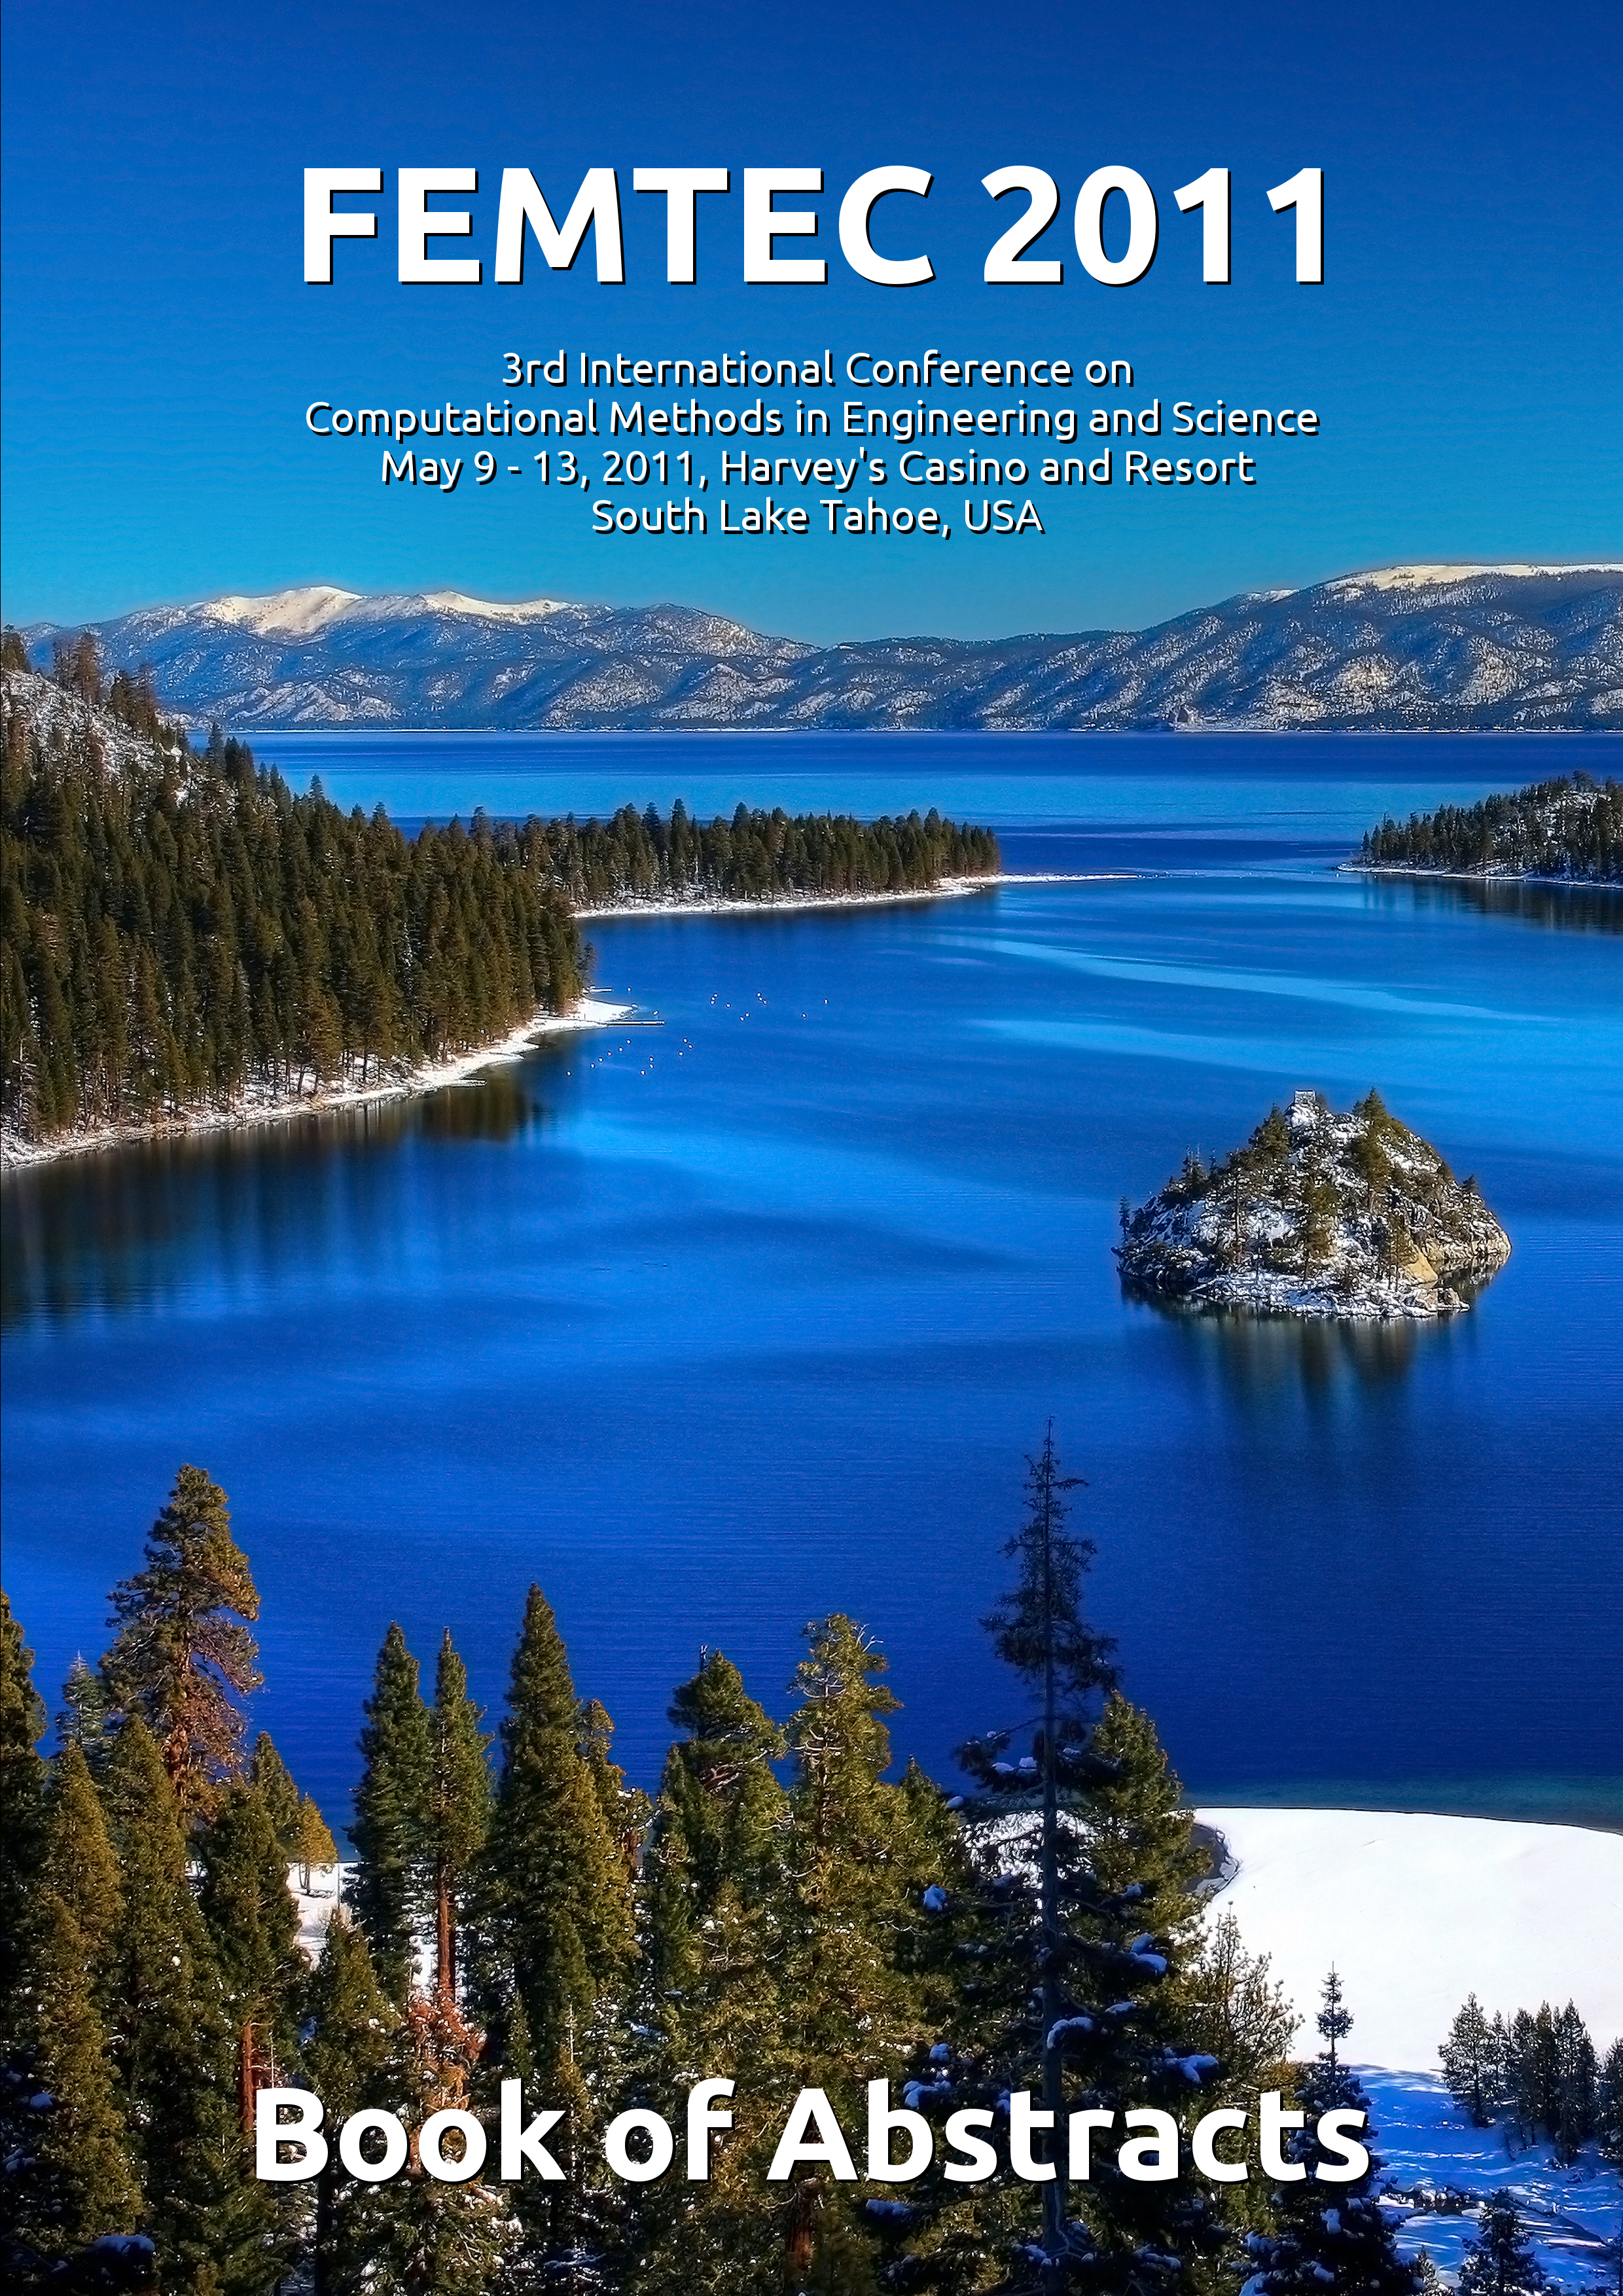
\includegraphics[width=\paperwidth,height=\paperheight]{img/background.jpg}
\vfill
}}}

\begin{document}

% INPUTTING BACKGROUND IMAGE
\AddToShipoutPicture{\BackgroundPic}
\vbox{}
\pagestyle{empty}
\newpage
\textwidth=15.5cm
\ClearShipoutPicture
\newpage

%%%%%%%%%%%%%%%%%%%%%%%%%%%%%%%%%%%%%%%%%%%%%%%%%%%%%%%%%%%%%%%%%%%%%%%%%

\section*{}
\small
\input ../common/aboutnclab.tex

\subsection*{Acknowledgement}
This publication was created with the help of numerous freely 
available web resources and tutorials related to Python, Scipy,
Numpy, Pylab, Matplotlib, Sympy and other projects.

\normalsize

\newpage
%{\ }
\setcounter{tocdepth}{2}
\tableofcontents
%\pagestyle{plain}

\newpage

\pagestyle{plain}
\setcounter{page}{1}

%%%%%%%%%%%%%%%%%%%%%%%%%%%%%%%%%%%%%%%%%%%%%%%%%%%%%%%%%%%%%%%%%%%%%%%%%



\section{Introduction}

All examples in this section are available in the displayed project 
"Math - Tutorial - 10 - Differential Equations". You can clone the project into 
your user account via the menu Project $\rightarrow$ Clone in the File 
Manager, and experiment with the examples on your own.
NCLab can solve Ordinary Differential Equations symbolically through the 
Sympy library. Remember that this library needs to be imported, and 
symbolic variables need to be declared:

\begin{verbatim}
from sympy import *
x, y, z = symbols("xyz")
\end{verbatim}
{\bf NOTE}: If you are looking for numerical methods to solve ODE, then
a vast amount is provided in the Scipy and Numpy libraries that can 
be imported in any Python worksheet. We refer to the web pages of these
two projects for details.

\section{Separable equations}

For example, let us solve the equation 
$$
  y'(x) + 9y(x) = 1.
$$
This is done as follows:
\begin{verbatim}
y = Function('f')
A = dsolve(diff(y(x), x) + 9*y(x) - 1, y(x))
pprint(A)
\end{verbatim}
Result:
\begin{verbatim}
/      9*x\      
|     e   |  -9*x
|C1 + ----|*e    
\      9  /    
\end{verbatim}
Another example: Let us solve the equation 
$$
  y'(x) = -xy(x).
$$
This is done as follows:
\begin{verbatim}
y = Function('f')
A = dsolve(diff(y(x), x) + y(x) * x, y(x))
pprint(A)
\end{verbatim}
Result:
\begin{verbatim}
      2
    -x 
    ---
     2 
C1*e   
\end{verbatim}

\section{Linear equations - homogeneous}
Linear equations are equations of the form 
$$
a(x) y'(x) + b(x) y(x) = g(x).
$$ 
They are called {\em homogeneous} if $g(x) = 0$.
An example:
$$
(x^2 - 9) y'(x) + x y(x) = 0.
$$
This is done as follows:
\begin{verbatim}
y = Function('f')
A = dsolve((x**2 - 9)*diff(y(x), x) + y(x) * x, y(x))
pprint(A)
\end{verbatim}
Result:
\begin{verbatim}
     C1    
-----------
   ________
  /      2 
\/  9 - x  
\end{verbatim}

\section{Linear equations - nonhomogeneous}

An example of a nonhomogeneous linear equations is
$$
(x^2 - 9) y'(x) + x y(x) = x^2.
$$
This is done as follows:
\begin{verbatim}
y = Function('f')
A = dsolve((x**2 - 9)*diff(y(x), x) + y(x) * x - x**2, y(x))
pprint(A)
\end{verbatim}
Result:
\begin{verbatim}
           /x\        ________
     9*asin|-|       /      2 
           \3/   x*\/  9 - x  
C1 - --------- + -------------
         2             2      
------------------------------
            ________          
           /      2           
         \/  9 - x            
\end{verbatim}

%\section{Laplace transform}



\section{Nonlinear equations}

For example, let us solve the equation 
$$
  y'(x) = x^2 y^2(x).
$$
This is done as follows:
\begin{verbatim}
y = Function('f')
A = dsolve(diff(y(x), x) + y(x)**2 * x**2, y(x))
pprint(A)
\end{verbatim}
Result:
\begin{verbatim}
1/(C1 + x**3/3)
\end{verbatim}

%%%%%%%%%%%%%%%%%%%%%%%%%%%%%%%%%%%%%%%%%%%%%%%%%%%%%%%%%%%%%%%%%%%%%%%%%





\end{document}
